% --------------------------------------------------------------
% This is all preamble stuff that you don't have to worry about.
% Head down to where it says "Start here"
% --------------------------------------------------------------

\documentclass[12pt]{article}
\usepackage{algorithm2e}
\usepackage{setspace}
\usepackage{enumerate}
\usepackage[mathscr]{euscript}
\usepackage{graphicx}
\usepackage{multicol}
\oddsidemargin 0.0in \textwidth 6.0in \textheight 9.0in \headsep
0.0in
\parskip 2mm
\parindent=0in
\pagestyle{empty}
\usepackage{color}
\usepackage{eurosym}
\usepackage{fullpage}
\usepackage{framed}
\usepackage{subcaption}
\usepackage{heuristica}

 \usepackage{amsmath}
\usepackage[utf8]{inputenc}
\usepackage[english]{babel}

\usepackage{amsthm}
\newtheorem{theorem}{Theorem}[section]
\newtheorem{lemma}[theorem]{Lemma}

%\thispagestyle{ucd}bibliography.bib
\usepackage{amsmath, amssymb}
\usepackage[utf8]{inputenc}
%\usepackage[english]{babel}
%\usepackage{natbib}
\bibliographystyle{apa}
\usepackage[backend=biber,style=numeric,sorting=ynt]{biblatex}
\addbibresource{review_template.bib}
\usepackage[dvipsnames]{xcolor}
\usepackage{hyperref}
\hypersetup{citecolor=blue,
    colorlinks=true,
    linkcolor=blue,
    filecolor=magenta,      
    urlcolor=blue,
    linktocpage=true
}

%\usepackage{natbib}% Citation support using natbib.sty
%\bibpunct[, ]{(}{)}{;}{a}{}{,}% Citation support using natbib.sty
%\renewcommand\bibfont{\fontsize{10}{12}\selectfont}% Bibliography support using natbib.sty

\newcommand{\N}{\mathbb{N}}
\newcommand{\Z}{\mathbb{Z}}
 
\newenvironment{theorem}[2][Theorem]{\begin{trivlist}
\item[\hskip \labelsep {\bfseries #1}\hskip \labelsep {\bfseries #2.}]}{\end{trivlist}}
\newenvironment{lemma}[2][Lemma]{\begin{trivlist}
\item[\hskip \labelsep {\bfseries #1}\hskip \labelsep {\bfseries #2.}]}{\end{trivlist}}
\newenvironment{exercise}[2][Exercise]{\begin{trivlist}
\item[\hskip \labelsep {\bfseries #1}\hskip \labelsep {\bfseries #2.}]}{\end{trivlist}}
\newenvironment{reflection}[2][Reflection]{\begin{trivlist}
\item[\hskip \labelsep {\bfseries #1}\hskip \labelsep {\bfseries #2.}]}{\end{trivlist}}
\newenvironment{proposition}[2][Proposition]{\begin{trivlist}
\item[\hskip \labelsep {\bfseries #1}\hskip \labelsep {\bfseries #2.}]}{\end{trivlist}}
\newenvironment{corollary}[2][Corollary]{\begin{trivlist}
\item[\hskip \labelsep {\bfseries #1}\hskip \labelsep {\bfseries #2.}]}{\end{trivlist}}
 
 

 
 
\begin{document}
\title{Statistical inference - Tutorial 3}%replace X with the appropriate number
\author{Estev\~ao B. Prado} %if necessary, replace with your course title
\maketitle

\section{Exercise 1}
1) We know that $\{X_{i}\}_{i=1}^{n} \sim \mbox{Negative Binomial}(r, p)$, where $r$ is known. We have that
\begin{equation}
f(x; r, p) = {x-1 \choose r - 1}p^{r} (1-p)^{x-r}.
\end{equation}

\subsection{Part a}
To solve this exercise, we'll use the definition of Exponential family distributions that's given in section 4.3 of \textbf{Sufficiency and the Rao-Blackwell Theorem} (weeks 6 and 7).

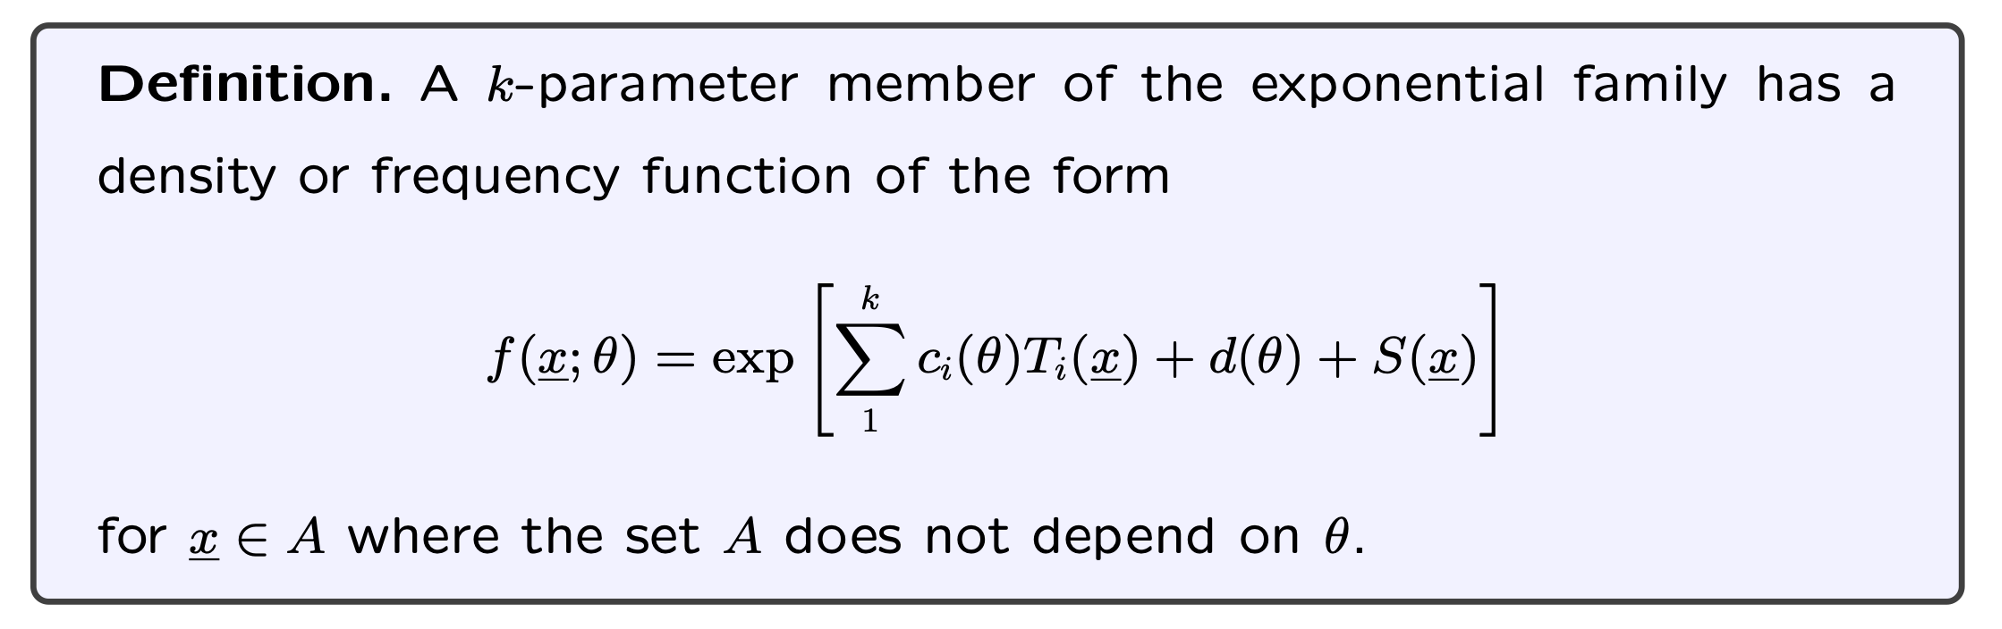
\includegraphics[width=1\linewidth]{Definition_exponential_family.png}

That is, we need to show that $f(x; r, p)$ has the same form of $f(x; \theta)$. For instance, we can rewrite $f(.)$ as follows.
\begin{align}
f(x; r, p) & = {x-1 \choose r - 1}p^{r} (1-p)^{x-r}, \\
& = \exp\left[ \log\left[ {x-1 \choose r - 1}p^{r} (1-p)^{x-r}\right] \right], \\
& = \exp\left[ \log {x-1 \choose r - 1} + r \log\left(p\right) + (x-r) \log\left( 1-p \right) \right], \mbox{by rule of log}, \\
& = \exp\left[ S(x) + d(p) + c(p)\times T(x) \right],
\end{align}
where $S(x) = \log {x-1 \choose r - 1}$, $d(p) = r \log(p)$, $c(p) = log(1-p)$ and $T(x) = x - r$, where $r$ is known.


\subsection{Part b}
We recall the Factorisation Theorem, which is introduced in section 4.1 (Sufficiency) on page 2.

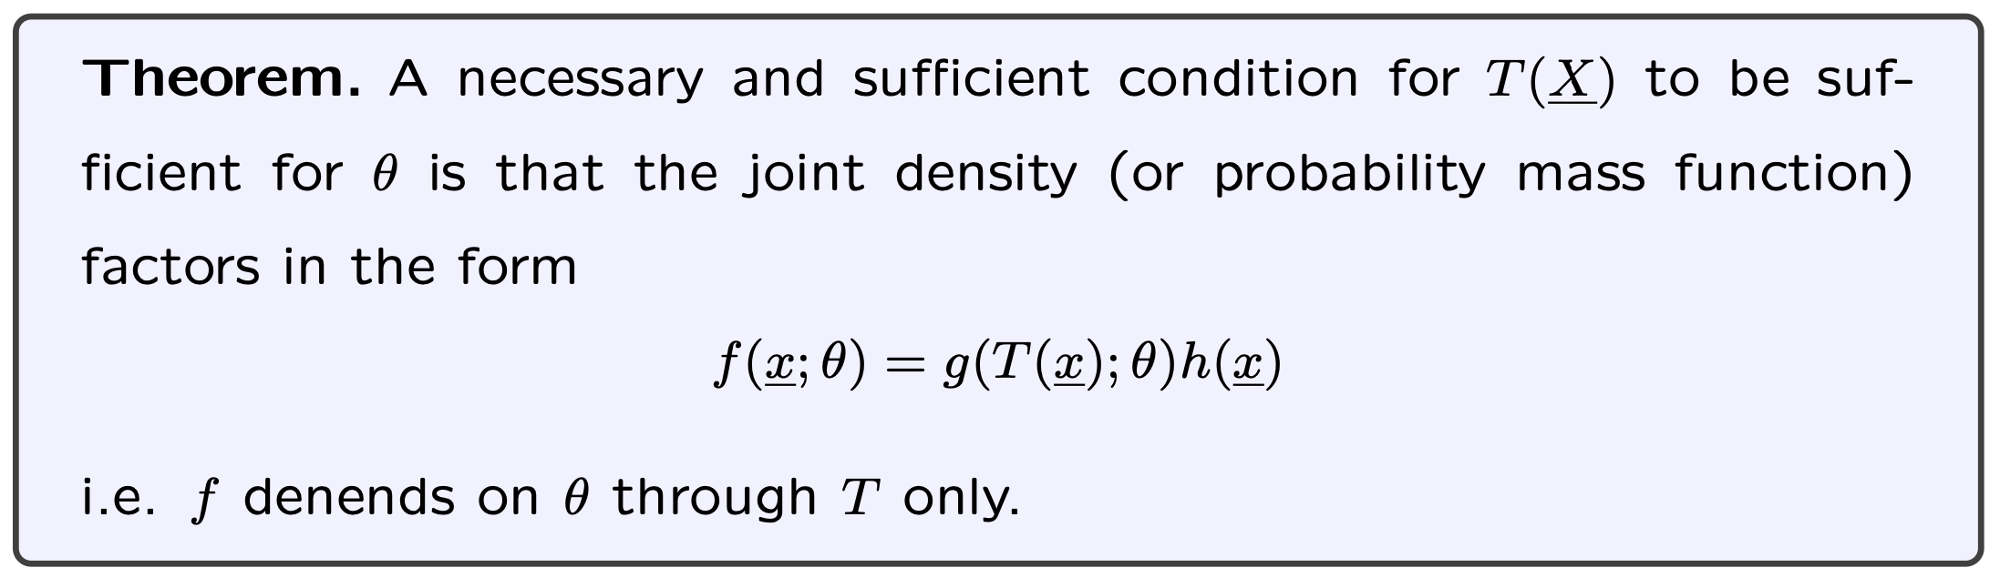
\includegraphics[width=1\linewidth]{Factorisation_theorem.png}

\begin{align}
\prod_{i=1}^{n} f(x_{i}; r, p) & = \prod_{i=1}^{n} {x_{i}-1 \choose r - 1}p^{r} (1-p)^{x_{i}-r}, \\
& = \prod_{i=1}^{n} \left[ {x_{i}-1 \choose r - 1} \right] p^{n r} (1-p)^{\sum_{i=1}^{n} (x_{i}-r)}, \\
& = p^{n r} (1-p)^{\sum_{i=1}^{n} (x_{i}-r)} \prod_{i=1}^{n} \left[ {x_{i}-1 \choose r - 1} \right], \\
& = g(T(\textbf{x}); p) h(\textbf{x}),
\end{align}
where $T(\textbf{x}) = \sum_{i=1}^{n} (x_{i}-r)$ is the sufficient statistics for $p$.

\section*{Exercise 3}

We know that $\{X_{i}\}_{i=1}^{n} \sim \mbox{Negative Binomial}(r, p)$, where $r$ is known. We have that
\begin{equation}
f(x; n, p) = {n \choose x}p^{x} (1-p)^{n-x}.
\end{equation}

\subsection*{Part a}
It's possible to answer this using two approaches: Factorisation Theorem or via a corollary of the Factorisation theorem, which uses the MLE. First, we use the FT as follows.

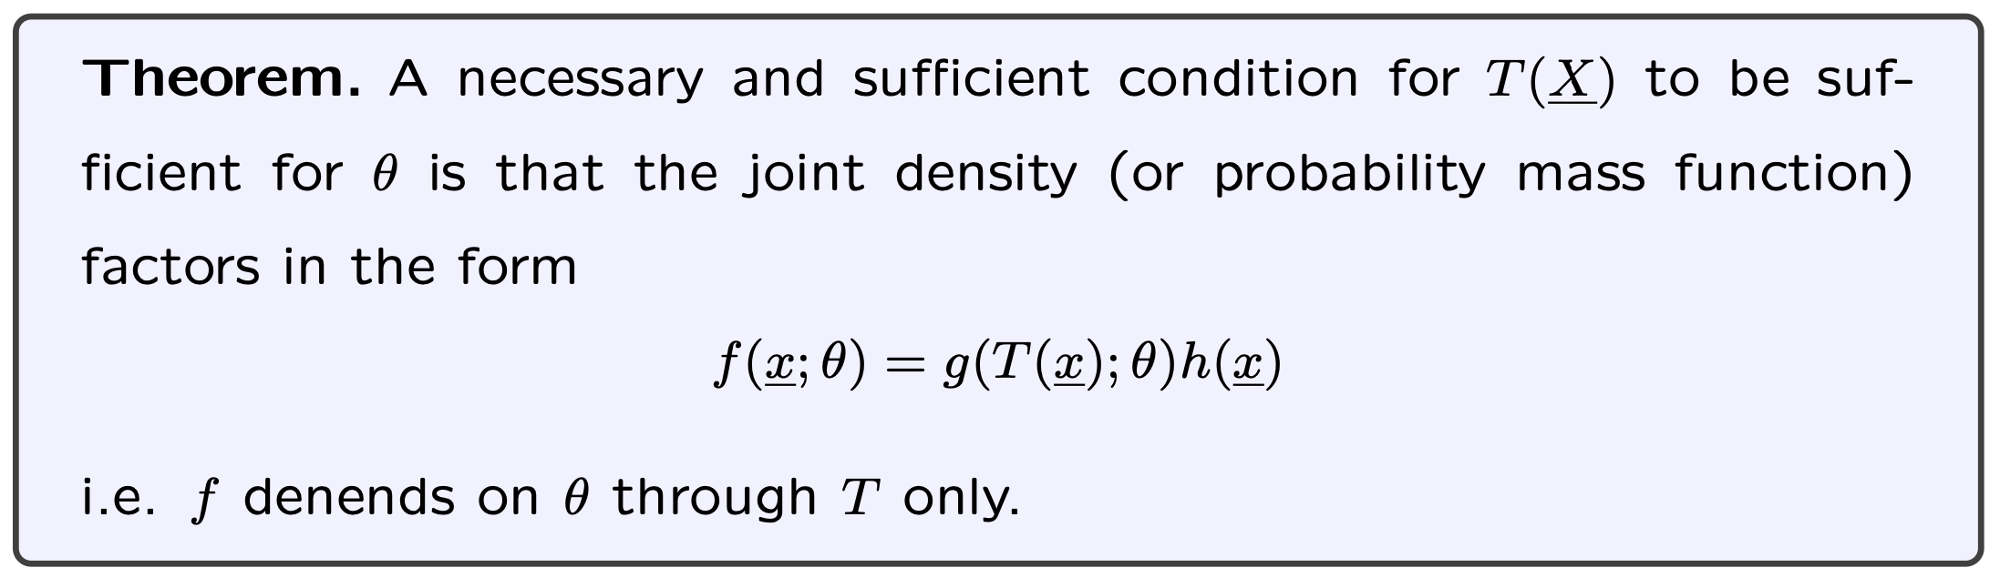
\includegraphics[width=1\linewidth]{Factorisation_theorem.png}

\begin{align}
\prod_{i=1}^{n} f(x_{i}; k, p) & = \prod_{i=1}^{n} {k \choose x_{i}}p^{x_{i}} (1-p)^{k-x_{i}}, \\
& = \prod_{i=1}^{n} \left[ {k \choose x_{i}} \right] p^{ \sum_{i=1}^{n} x_{i}} (1-p)^{\sum_{i=1}^{n} (k-x_{i})}, \\
& = p^{\sum_{i=1}^{n} x_{i}} (1-p)^{ nk- \sum_{i=1}^{n}x_{i}} \prod_{i=1}^{n} \left[ {k \choose x_{i}} \right], \\
& = g(T(\textbf{x}); p) h(\textbf{x}),
\end{align}
where $T(\textbf{x}) = \sum_{i=1}^{n} x_{i}$ is the sufficient statistics for $p$.

Another possibility is to use a corollary of the Factorisation theorem. To use it, we first need to find the MLE of the parameter of interest ($p$). 

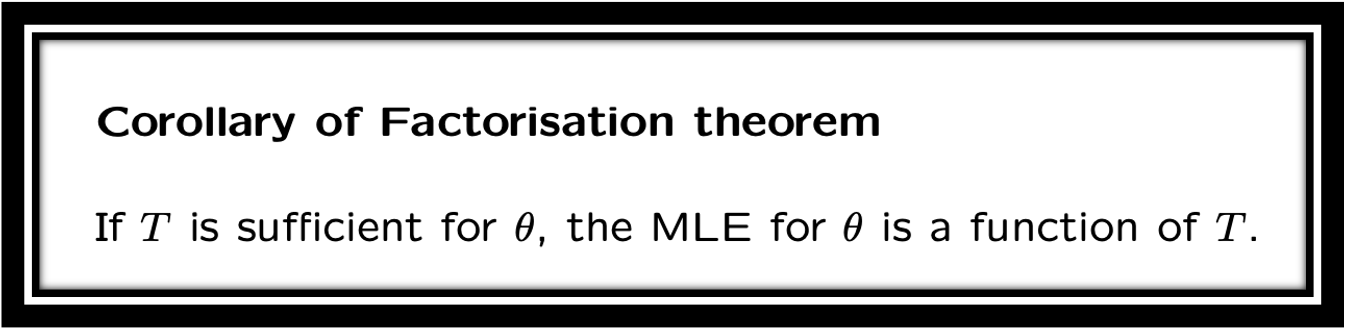
\includegraphics[width=1\linewidth]{corollary_factorisation_theorem.png}

Here, we know that the MLE is $\hat{p} = \sum_{i=1}^{n}x_{i}/nk$. Hence, as the sufficient statistics $T$ is a function of $\hat{p}$, we conclude that $T = \sum_{i=1}^{n}x_{i}$, as $n$ and $k$ are known.

\subsection*{Part b}

First, we know that $\mathbb{E}(X_{i}) = kp$ and $\mathbb{V}(X_{i}) = kp(1-p)$. Again, there are two ways to answer this. For instance, we could show that $\hat{p}$ is an unbiased estimator (i.e., $\mathbb{E}(\hat{p})= p$) and that $\mathbb{V}(\hat{p})$ attains the Cramer-Rao Lower bound. I guess this is the easiest way to show what we need.

The second alternative is to use the Lehmann-Scheffe Theorem.

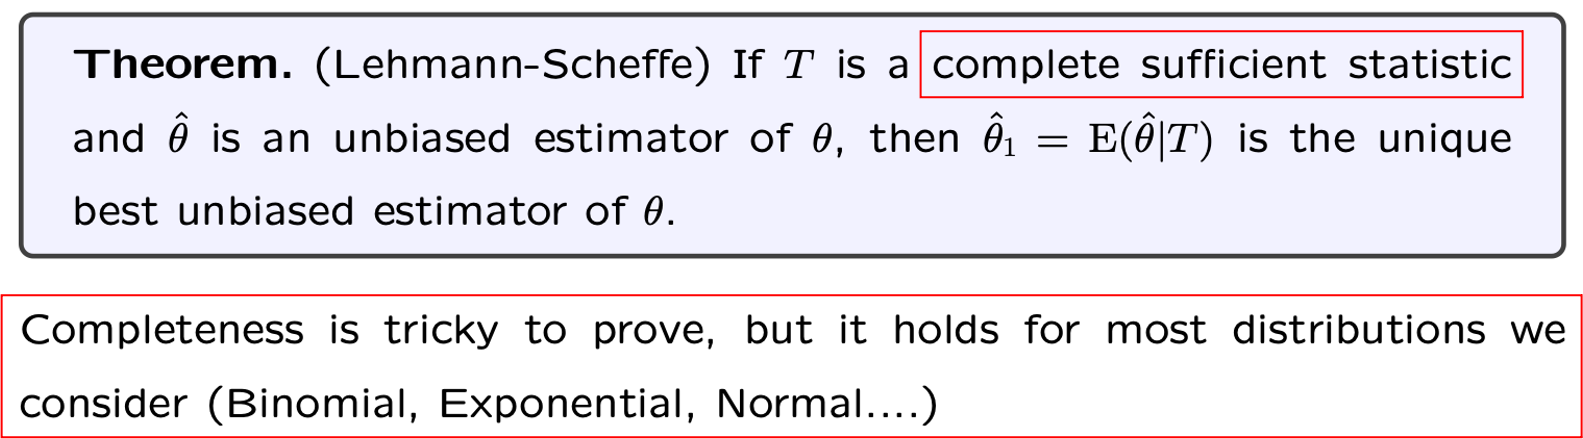
\includegraphics[width=1\linewidth]{Leman_theorem.png}

We know that $\hat{p} = \sum_{i=1}^{n}x_{i}/nk$ is unbiased because
\begin{align}
\mathbb{E}(\hat{p}) & = \mathbb{E}\left(\frac{\sum_{i=1}^{n}X_{i}}{nk}\right), \\
& = \frac{\sum_{i=1}^{n} \mathbb{E}(X_{i}) }{nk} , (X_{i}'s \mbox{ are i.i.d})\\
& = \frac{n \mathbb{E}(X_{i}) }{nk} , (X_{i}'s \mbox{ are i.i.d}) \\
& = \frac{\mathbb{E}(X_{i}) }{k} , \\
& = \frac{kp}{k}, \\
& = p.
\end{align}
In addition, recall that in a) we found that $T = \sum_{i=1}^{n}x_{i}$ is a sufficient statistics for $p$. However, by the Lehmann-Scheffe Theorem $T$ is a \textbf{complete sufficient statistics} for $p$ because the completeness of sufficient statistics holds for all distributions that belong to the exponential family (see section 4.3, page 6), which is the case of the Binomial distribution. Consequently, if $\mathbb{E}(\hat{p})$ is unbiased estimator and $T$ is a \textbf{complete sufficient statistics}, then $\hat{p}$ is BUE.

\subsection*{Part c}

To answer this, we need to get back all the way to weeks 2 and 3 (MLE, page 9) and refresh our memory about the Invariance property of the MLE.

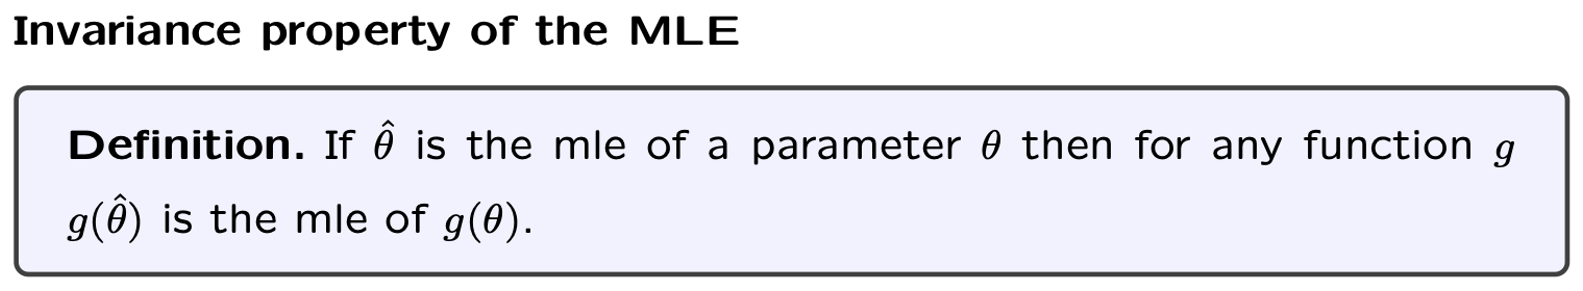
\includegraphics[width=1\linewidth]{invariance.png}

That is, the MLE for $g(p) = kp(1-p)^{k-1}$ is $g(\hat{p}) = k\hat{p}(1-\hat{p})^{k-1}$, where $\hat{p} = \sum_{i=1}^{n}x_{i}/nk$.

\subsection*{Part d}

First, we'll take the hint and we'll consider an unbiased estimator of $g(p)$ in the form of
\begin{equation} \tilde{g(p)} = 
    \begin{cases}
      1, \mbox{if } X_{1} = 1 \\
      0, \mbox{otherwise}. 
    \end{cases}
\end{equation}

Hence, we can check that 

\begin{align}
\mathbb{E}(\tilde{g(p)}) & = 1 \times p(X_{1}=1) + 0 \times p(X_{1} \ne 1), \\
& = p(X_{1}=1), \\ 
& = g(p).
\end{align}

In addition, we know from a) that $T = \sum_{i=1}^{n} x_{i}$ and that consequently $T \sim \mbox{Binomial}(nk, p)$. Now, let's recall the Rao-Blackwell Theorem.

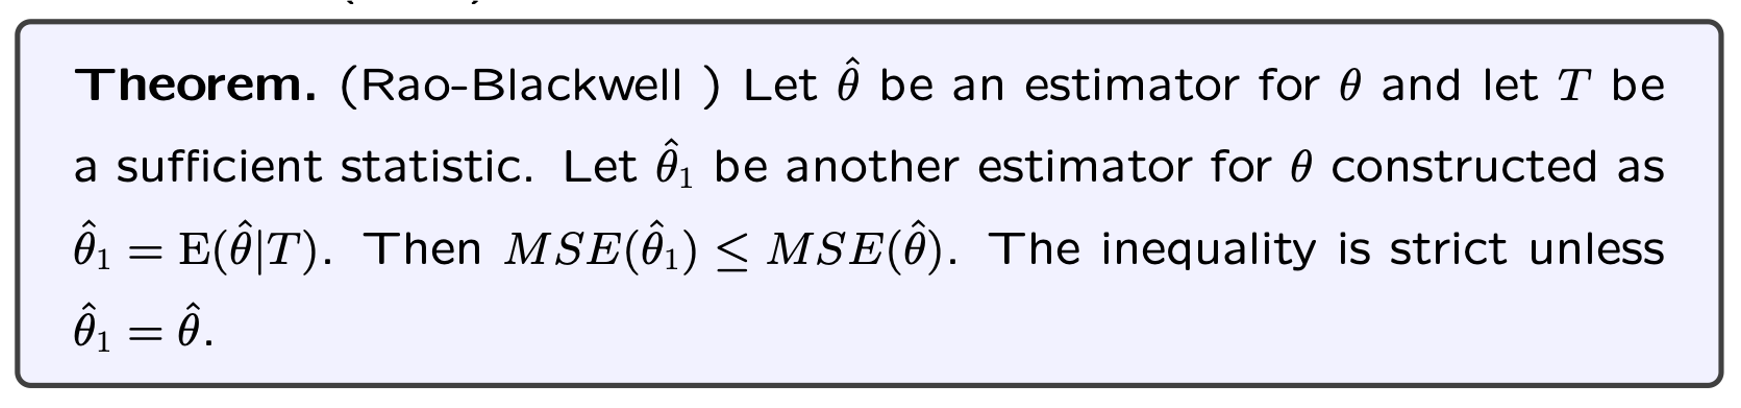
\includegraphics[width=1\linewidth]{rao_blackwell.png}

Based on the theorem above, we have an estimator for $g(p)$, which $\tilde{g(p)}$, and we have a sufficient statistics $T = \sum_{i=1}^{n}x_{i}$. Still according to the theorem, a natural estimator for $g(p)$ is given by $\mathbb{E}(\tilde{g(p)}|T)$. We know that

\begin{align}
\mathbb{E}(\tilde{g(p)}|T) & = p(X_{1} = 1| T = t), \\
& = \frac{p(T = t|X_{1} = 1) p(X_{1} = 1)}{P(T=t)}, \mbox{due to Bayes' theorem} \\
& = \frac{p(T = t - 1) p(X_{1} = 1)}{P(T=t)}, \\
& = \frac{\mbox{Binomial}(t-1; n-1, p) kp(1-p)^{k-1}}{\mbox{Binomial}(t; n, p)} \\
& = \frac{{(n-1)k \choose t-1} k}{{nk \choose t}}.
\end{align}

Along with the Lehmann-Scheffe Theorem, we have that $\mathbb{E}(\tilde{g(p)}|T)$ is BUE for $g(p)$.

\end{document}